\chapter{Analisis}
\label{chap:analysis}
Pada bab ini, akan dijelaskan mengetai analisis kebutuhan dan fitur perangkat lunak, Diagram pengembangan perangkat lunak, \textit{use case} dari perangkat lunak serta diagram aktifitas dari perangkat lunak.
\section{Analisis Kebutuhan dan Fitur Perangkat Lunak}
\subsection{Analisis Kebutuhan}
Pertama-tama modul BI ini terintegrasi dengan ODOO, sebelum menggunakan modul ini maka pengguna diwajibkan untuk menginstall ODOO. Berikut ini \textit{requirement component} yang diperlukan untuk menginstall ODOO:
\begin{enumerate}
	\item \textit{installer} ODOO 8.0-20141128
	\item PosgreSQL 9.3
	\item Phyton 2.7
\end{enumerate} 
Sedangkan untuk minimum \textit{requirement hardware}, yaitu: 
\begin{enumerate}
	\item Intel x86 atau x64
	\item Minimum RAM 512 MB
	\item Minimum ruang di hardisk 150 MB
	\item Mendukung protokol TCP/IP
	\item OS x86 atau x64 MAC, Linux, atau Windows
\end{enumerate}
 
\subsection{Fitur Perangkat Lunak}
Perangkat Lunak ini akan memiliki fitur seperti gambar \textbf{3.1} :
\begin{figure}[h]
	\centering
	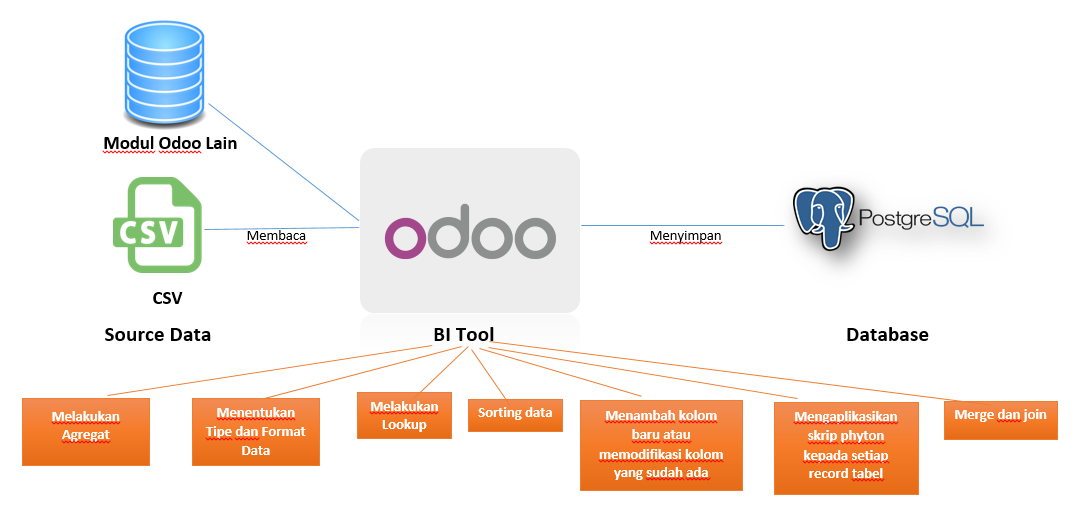
\includegraphics[scale=0.5]{Gambar/fitur-bi-tool}
	\caption{Fitur BI \textit{tool}}
	\end{figure}
	
	\begin{enumerate}
		\item BI \textit{tool} menerima dan membaca \textit{input source} berupa CSV/\textit{text file}, dan modul ODOO lain.
		\item Dapat menentukan tipe dan format data
		\item Dapat melakukan \textit{Lookup}
		\item Dapat melakukan agregat
		\item Dapat melakukan \textit{sorting} data
		\item Dapat menambah kolom baru atau memodifikasi kolom yang sudah ada
		\item Dapat mengaplikasikan skrip phyton terhadap setiap baris \textit{record}
		\item Dapat melakukan \textit{merge} dan \textit{join}
		\item Data yang telah diproses dapat disimpan dalam \texttt{database}
	\end{enumerate}
	
\subsection{Diagram Aktifitas pada BI \textit{Tool}}
	Pada subbab ini akan dibahas mengenai prosedur setiap aktifitas dari fitur yang diberikan oleh BI \textit{tool}.
	
	\subsubsection{Membuat Bisnis Baru}
	Sebelum melangkah pada proses ETL pengguna diwajibkan membuat nama bisnis untuk membedakan setiap proses ETL.
	Berikut ini step-step untuk membuat bisnis baru.
	\begin{figure}[h]
	\centering
	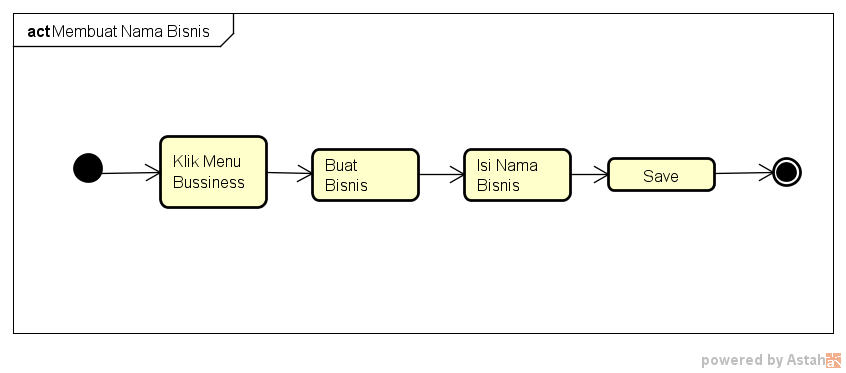
\includegraphics[scale=0.7]{Gambar/Membuat-Nama-Bisnis}
	\caption{Prosedur Membuat Bisnis Baru}
	\end{figure}
	
	\begin{enumerate}
		\item Pengguna mengklik menu \textit{Businesses}.
		\item Pengguna membuat nama bisnis baru.
		\item Pengguna mengisi kolom nama bisnis.
		\item Setelah selesai lalu pengguna mengklik tombol save.
	\end{enumerate}
	
	
	\subsubsection{Memasukan \textit{Data Source}}

	\begin{figure}[h]
	\centering
	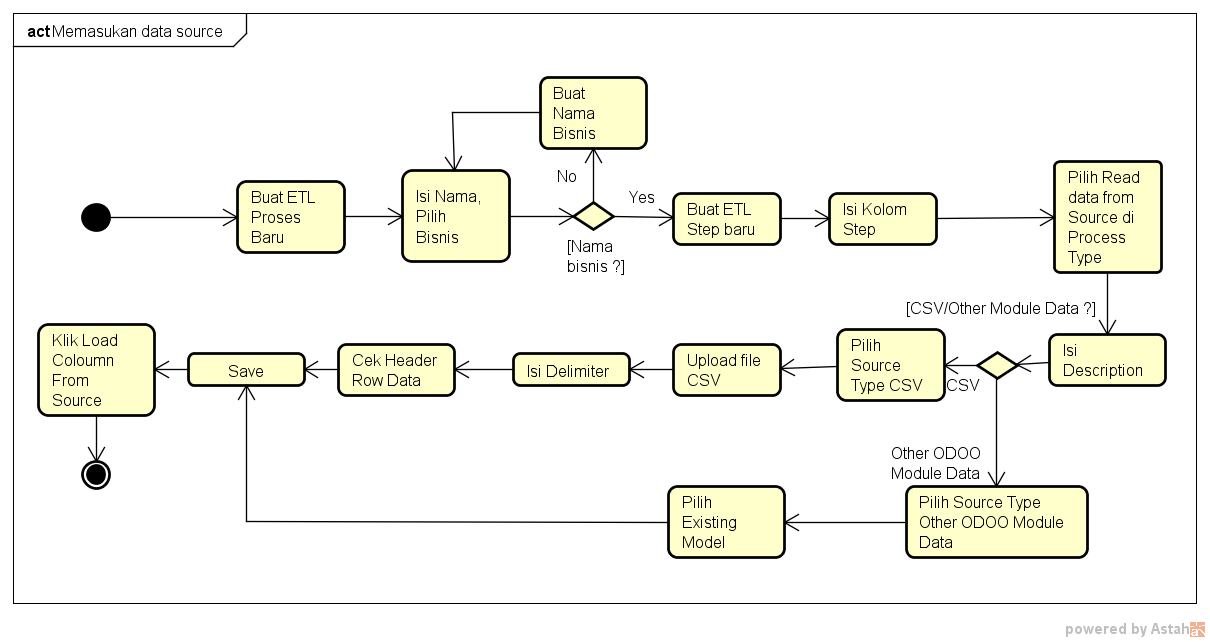
\includegraphics[scale=0.5]{Gambar/Memasukan-data-source}
	\caption{Prosedur Memasukan \textit{Data Source}}
	\end{figure}
	
	Pengguna dapat memasukan \textit{data source} bertipe CSV/\textit{teks file} atau modul ODOO lain dan menggunakannya sebagai sumber data untuk
	tipe proses lain dari fitur BI. Berikut tahapan-tahapan bagaimana memasukan data kedalam BI \textit{tool}.
	\begin{enumerate}
		\item Pengguna mengakses menu ETL \textit{Process} dan membuat proses ETL baru dengan menuliskan nama pada kolom nama yang tersedia.
		\item Selanjutnya pengguna memilih tipe bisnis yang telah dibuat sebelumnya, bila pengguna belum membuatnya maka pengguna dapat membuat nama bisnis terlebih dahulu sebelum melangkah ke proses selanjutnya.
		\item setelah kolom bisnis terisi maka pengguna membuat baru step etl 
		\item sesudahnya pengguna menuliskan nomer step untuk menentukan urutan \textit{compile} oleh BI \textit{tool}
		\item Pengguna memilih pilihan \textit{read data from source} dikolom \textit{process type} dilanjutkan dengan menuliskan deskripsi prosesnya pada kolom \textit{description}
		\item Pengguna dapat memilih tipe \textit{input} CSV atau Modul ODOO lain.
		\item Jika pengguna memilih tipe data CSV maka pada kolom \textit{source type} pilih CSV.
		\item Selanjutnya, Pengguna meng-\textit{upload} data CSV pada tempat yang disediakan
		\item Pengguna lalu mengisi kolom \textit{delimiter} dilanjutkan dengan menceklis kolom \textit{header row present?} bila baris pertama sumber data CSV adalah judul kolom.
		\item Jika pengguna memilih modul ODOO lain maka pada kolom \textit{source type} pilih \textit{other ODOO module data}.
		\item Setelah itu, pengguna memilih modul yang telah terinstal dalam odoo yang akan dijadikan \textit{source}.
		\item Setelah proses memilih \textit{source} selesai, Pengguna mengklik tombol \textit{save}, lalu mengklik kembali tombol \textit{load columns from source} untuk mengambil semua alamat kolom dalam \textit{source} untuk digunakan pada tipe proses selanjutnya.
	\end{enumerate}
	
\subsubsection{Menentukan Tipe dan Format Data}

	\begin{figure}[h]
	\centering
	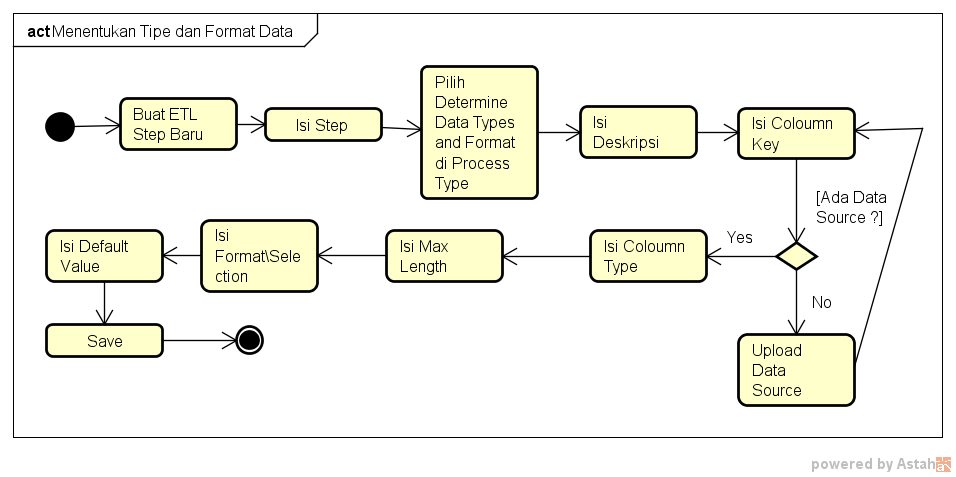
\includegraphics[scale=0.5]{Gambar/Menentukan-Tipe-dan-Format-Data}
	\caption{Prosedur Menentukan Tipe dan Format Data}
	\end{figure}

	Pengguna dapat menentukan tipe dan format data sesuai keinginan, namun syaratnya adalah \textit{data source} sudah di upload kedalam BI \textit{tool}. Berikut ini prosedur menentukan tipe data serta memformat data.
	\begin{enumerate}
		\item Membuat step ETL baru pada menu \textit{ETL process}.
		\item kemudian menuliskan nomer step pada kolom step, karena step pertama di isi oleh \textit{input data source} maka kolom step diisi oleh nomer yang lebih besar dari satu.
		\item Memilih \textit{determine data types and format} di kolom \textit{Process type}, dilanjutkan dengan mengisi kolom deskripsi.
		\item Selanjutnya mengisi \textit{Column key} 
		\item Dilanjutkan dengan mengisi \textit{column type}
		\item lalu menuliskan \textit{max length} untuk membatasi isi dari \textit{field} tersebut.
		\item Pengguna menuliskan \textit{format/selection} dari agar format data seragam dan terstandarisasi.
		\item Pengguna juga dapat mengisi kolom \textit{default value} bila diperlukan.
		\item Setelah proses selesai lalu pengguna mengklik tombol save dan semua setinggan yang telah dimasukan pengguna akan tersimpan dalam \textit{database}.
	\end{enumerate}
	
\subsubsection{Melakukan \textit{Lookup}}

	\begin{figure}[H]
	\centering
	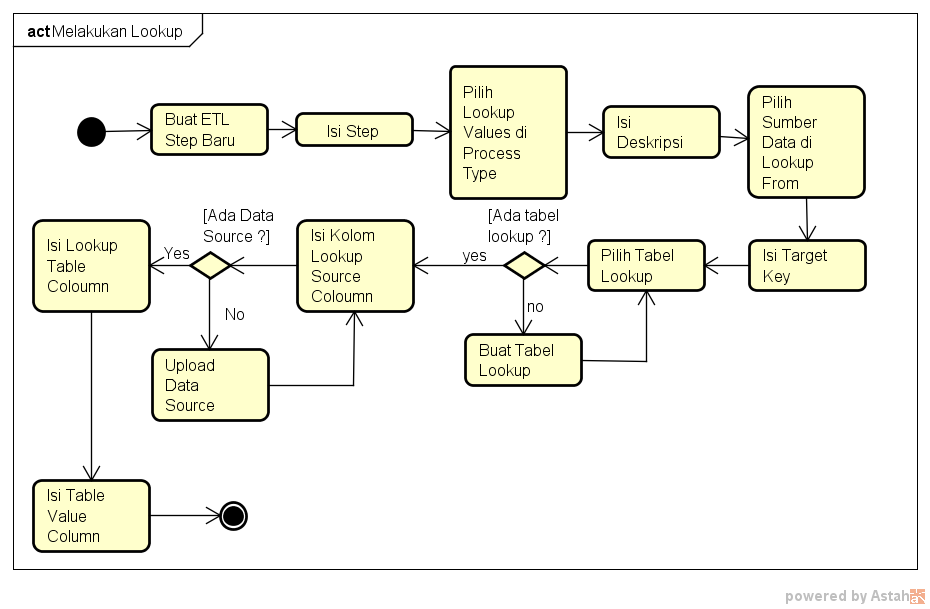
\includegraphics[scale=0.5]{Gambar/Melakukan-Lookup}
	\caption{Prosedur Melakukan \textit{Lookup}}
	\end{figure}

	Pengguna dapat melakukan \textit{lookup} dengan syarat \textit{data source} telah dimasukan kedalam \textit{database} BI tool. Berikut pemaparan proses penggunaan \textit{lookup}.
	\begin{enumerate}
		\item Pengguna membuat ETL step baru dengan mengisi nomer urutan dikolom step.
		\item Pengguna memilih \textit{process type} \textit{lookup values} serta menulis deskripsi step tersebut.
		\item Pengguna dapat memilih melakukan proses \textit{lookup} dengan tabel yang sudah ada didalam basis data BI tool atau menuliskan tabel baru pada kolom \textit{lookup value} dan \textit{result value}.
		\item pengguna menuliskan target \textit{field} yang akan disi.
		\item kemudian memilih \textit{value} kolom mana yang dijadikan acuan.
		\item setelah selesai pengguna mengklik tombol save untuk menyimpan setingan yang telah dimasukan sebelumnya.
	\end{enumerate}

\subsubsection{Melakukan \textit{Sorting Data}}
	\begin{figure}[H]
	\centering
	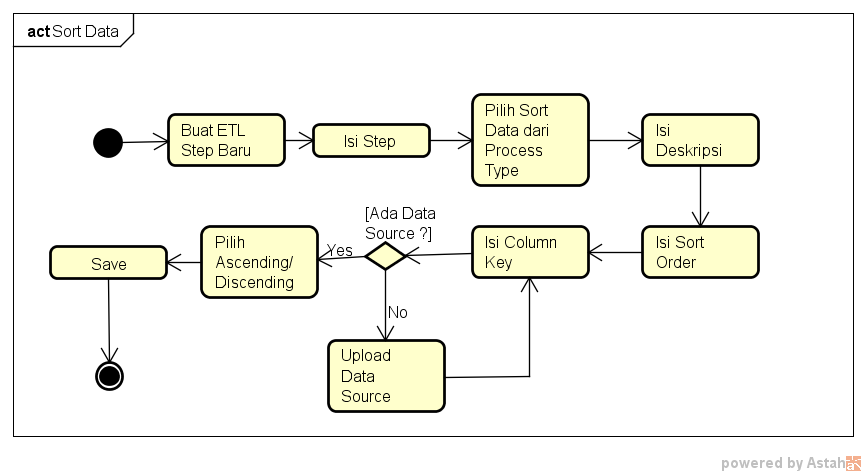
\includegraphics[scale=0.5]{Gambar/Sort-Data}
	\caption{Prosedur Melakukan \textit{Sorting Data}}
	\end{figure}
	
	Pada bagian ini pengguna dapat melakukan \textit{sorting data} dengan meng-\textit{input} sumber data terlebih dahulu. 
	Berikut penjelasan proses \textit{sort order}
	\begin{enumerate}
		\item Pengguna membuat ETL step baru dengan mengisi nomer urutan dikolom step.
		\item Selanjutnya memilih \textit{process type sort data} dilanjutkan dengan mengisi deskripsi proses tersebut.
		\item Pengguna menuliskan \textit{sort order} sesuai dengan urutan \textit{sort} yang terlebih dahulu di inginkan.
		\item Pengguna menuliskan \textit{column key} menandakan kolom \textit{source} mana yang akan diurutkan.
		\item Terakhir pengguna memilih \textit{direction} dari \textit{sort} yang di inginkan apakah \textit{ascending} atau \textit{descending}, lalu klik tombol \textit{save} untuk menyimpan semua \textit{setting} yang telah dilakukan.
	\end{enumerate}
	
\subsubsection{Menambah atau Memodifikasi Kolom}
	\begin{figure}[H]
	\centering
	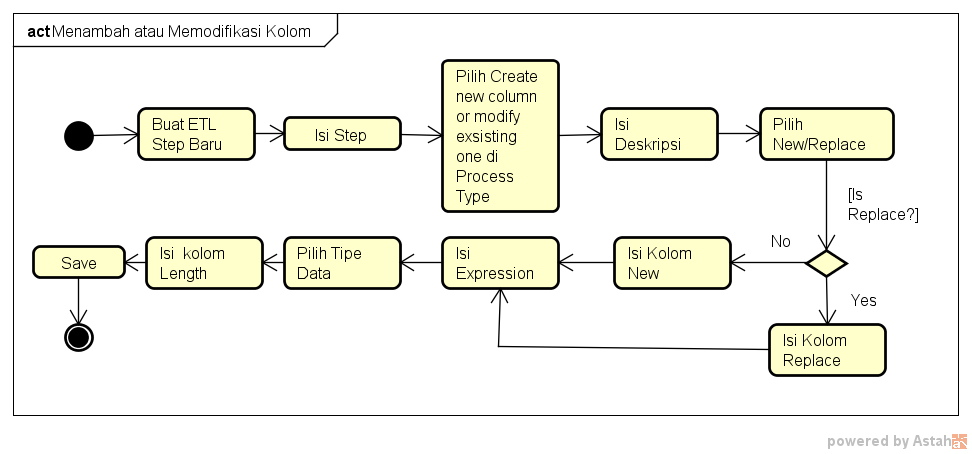
\includegraphics[scale=0.5]{Gambar/Menambah-atau-Memodifikasi-Kolom}
	\caption{Prosedur Menambah atau Memodifikasi Kolom}
	\end{figure}

	Pengguna dapat menambahkan kolom atau memodifikasi kolom yang tersedia dengan proses sebagai berikut.
	\begin{enumerate}
		\item Pengguna terlebih dahulu membuat ETL proses baru dan mengisi kolom step,
		\item Selanjutnya memilih \textit{create new column or modify existing one} pada kolom \textit{process type} dan menuliskan deskripsi dari proses tersebut.
		\item Pengguna menentukan apakan ingin menambahkan kolom baru atau memodifikasi kolom yang tersedia.
		\item Jika memodifikasi kolom tentukan kolom yang akan dimodifikasi.
		\item Jika membuat kolom baru pengguna menuliskan nama kolom baru.
		\item Setelah itu pengguna dapat menuliskan fungsi pyton untuk perhitungan atau tujuan lain pada kolom \textit{expression}.
		\item Pengguna menentukan tipe data kolom tersebut.
		\item Pengguna dapat menentukan panjang data yang akan dimasukan pada kolom \textit{length}.
		
	\end{enumerate}
	
\subsubsection{Mengaplikasikan Phyton \textit{Script}}

	\begin{figure}[H]
	\centering
	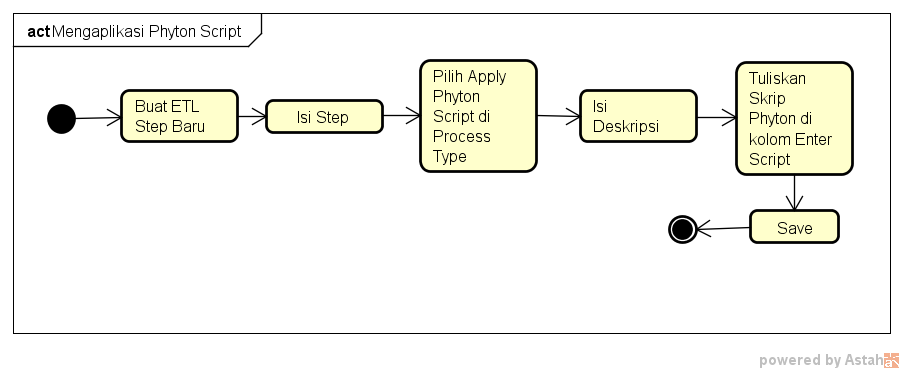
\includegraphics[scale=0.5]{Gambar/Mengaplikasikan-Phyton-Script}
	\caption{Prosedur Mengaplikasikan Phyton \textit{Script}}

	\end{figure}
	Pengguna dapat menjalankan skrip phyton yang berlaku untuk setiap baris data yang pada \textit{source}.
	Berikut proses memasukan skrip phyton pada BI \textit{tool}.
	\begin{enumerate}
		\item Pengguna membuat ETL step baru dengan mengisi nomer urutan dikolom step.
		\item Selanjutnya memilih \textit{process type apply phyton script to each data line} dilanjutkan dengan mengisi deskripsi proses tersebut.
		\item Setelah itu pengguna dapat langsung memasukan skrip phyton pada kolom \textit{enter script} pada perangkat lunak.
		\item Setelah selesai pengguna mengklik tombol save untuk menyimpan semua \textit{setting}.
	\end{enumerate}
	
\subsubsection{Melakukan Agregat}

	\begin{figure}[H]
	\centering
	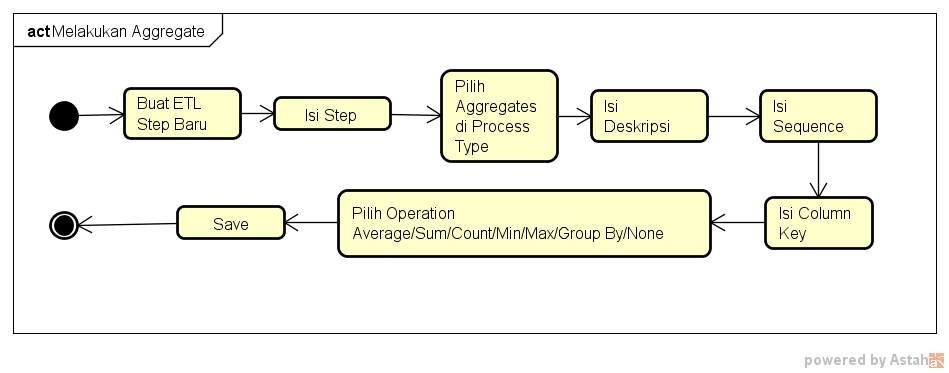
\includegraphics[scale=0.5]{Gambar/Melakukan-Aggregate}
	\caption{Prosedur Melakukan \textit{Aggregate}}
	\end{figure}	
	
	Pengguna dapat melakukan agregat terhadap \textit{data source}. Berikut pemaparan proses agregat.
	\begin{enumerate}
		\item Pengguna membuat ETL step baru dengan mengisi nomer urutan dikolom step.
		\item Pengguna memilih \textit{aggregates} pada kolom \textit{process type} dan menuliskan deskripsi mengenai proses tersebut.
		\item Pengguna menuliskan urutan dari pengerjaan agregat pada kolom \textit{sequence}.
		\item Pengguna memilih kolom yang akan di agregat.
		\item Pengguna memilih operasi yang dilakukan apakah \textit{count, max, min, sum, average, group by} ataupun \textit{none}.
		\item Setelah selesai pengguna mengklik tombol \textit{save}.
	\end{enumerate}
	
\subsubsection{Melakukan \textit{Merge Join}}

	\begin{figure}[H]
	\centering
	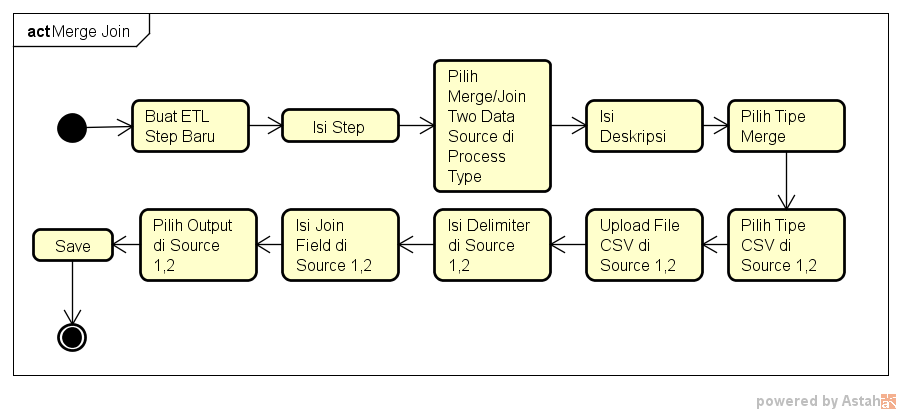
\includegraphics[scale=0.5]{Gambar/Merge-Join}
	\caption{Prosedur Melakukan \textit{Merge Join} dari dua \textit{data source}}
	\end{figure}

	Pengguna dapat melakukan \textit{merging} terhadap dua \textit{data source} sekaligus. Berikut pemaparan prosesnya. 
	\begin{enumerate}
		\item Pengguna membuat ETL step baru dengan mengisi nomer urutan dikolom step.
		\item Setelah itu memilih \textit{merge/join two data source} pada kolom \textit{process type} dan menuliskan deskripsi proses tersebut pada kolom \textit{description}.
		\item Pengguna memilih tipe \textit{merge} yang akan digunakan, yaitu \textit{left outer join}, \textit{inner join}, atau \textit{right outer join}.
		\item Pengguna menentukan tipe \textit{source}.
		\item Pengguna \textit{upload data source} jika tipe masukannya CSV.
		\item Pengguna mengisi kolom \textit{delimiter} jika tipe masukannya CSV.
		\item Setelah \textit{upload} selesai maka kolom pada \textit{source} akan terbaca otomatis oleh BI \textit{tool}.
		\item Setelah \textit{source} pertama selesai, pengguna melakukan step yang sama terhadap \textit{source} ke=2.
		\item Setelah kedua \textit{source} sudah terbacaa oleh BI tool, selanjutnya pengguna menuliskan \textit{join field} pada kedua kolom \textit{source} tersebut.
		\item Pengguna dapat menentukan \textit{output} kolom dengan menceklis mana saja yang akan menjadi \textit{output} dalam tabel destinasi pada bagian \textit{output} dalam BI \textit{tool}.
		\item Setelah semua selesai maka pengguna mengklik tombol \textit{save}.
	\end{enumerate}
	
	\subsubsection{\textit{Save to Database}}
	
	\begin{figure}[H]
	\centering
	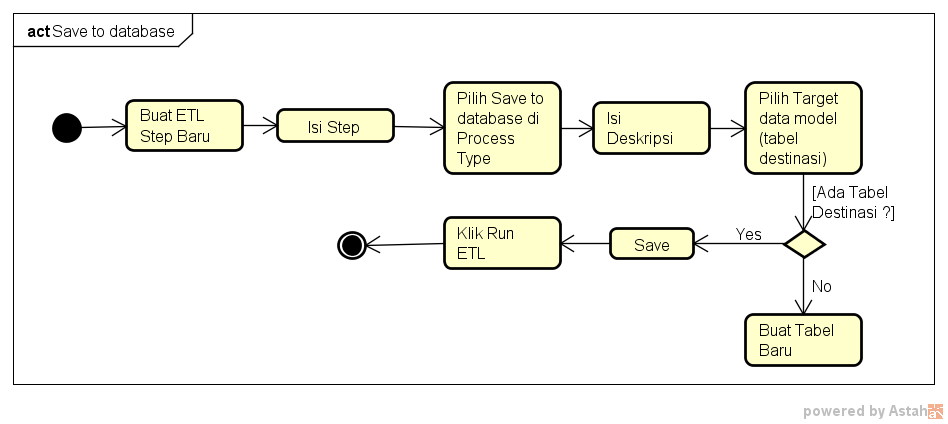
\includegraphics[scale=0.5]{Gambar/Save-to-database}
	\caption{Prosedur Menyimpan Data dalam \textit{Database}}
	\end{figure}
	
	Setelah semua tipe proses dilalui maka pengguna perlu menyimpan data hasil proses kedalam \textit{database} BI \textit{tool}. Namun, pastikan semua \textit{process type} telah terisi dengan benar, bila tidak hasil proses ETL tidak akan tersimpan dalam \textit{database}.  Untuk menyimpan data hasil proses kedalam tabel destinasi dalam \textit{database} syaratnya perlu minimal satu tipe proses \textit{read data from source} atau \textit{merge join} yang meminta \textit{input data source} pada pengguna. Berikut pemaparan lebih lanjut mengenai prosesnya.
\begin{enumerate}
	\item Pengguna membuat ETL step baru dengan mengisi nomer urutan dikolom step.
	\item Selanjutnya pengguna memilih \textit{save to database} pada kolom \textit{process type} dan menuliskan deskripsi singkat mengenai proses tersebut.
	\item Pengguna menentukan tabel destinasi tempat penyimpanan, dalam istilah ODOO disebut \textit{target data model}.
	\item Kolom destinasi akan terbaca secara otomatis oleh BI \textit{tool} setelah menentukan tabel destinasi/\textit{target data model}.
	\item Pengguna melakukan \textit{mapping} kolom dari \textit{source} mana yang akan masuk dalam tabel destinasi.
	\item Setelah semua selesai klik \textit{save}.
	\item Lalu, pengguna mengklik tombol \textit{Run ETL} untuk menjalankan semua tipe proses ETL dan menyimpannya dalam \textit{database}
\end{enumerate}
	
\section{Permodelan Tool}

Berikut diagram use case berserta skenario yang tertera pada gambar \textbf{3.10}

\begin{figure}[h]
	\centering
	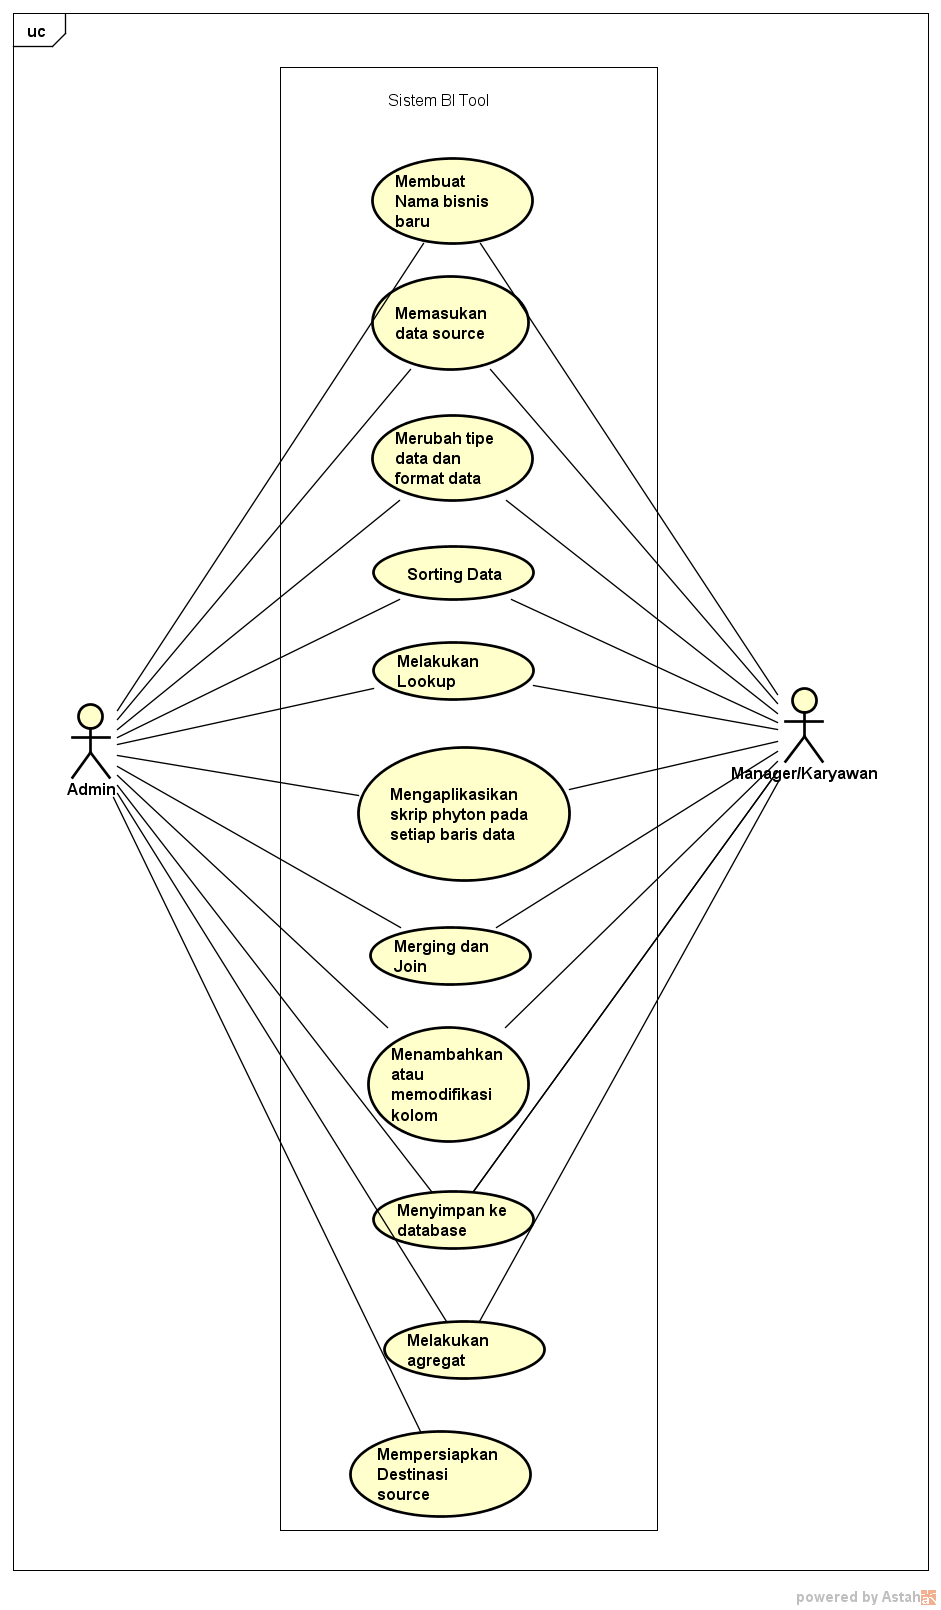
\includegraphics[scale=0.4]{Gambar/usecase-bi}
	\caption{Diagram use case BI \textit{tool}}
	\end{figure}

\begin{enumerate}
	\item Skenario Membuat Bisnis Baru \\
	{\renewcommand\labelitemi{}
		\begin{itemize}
			\item Deskripsi		: Kegiatan membuat nama bisnis.
			\item Aktor				: Admin, manajer
			\item Prakondisi	: -
			\item Skenario		:
				\begin{itemize}
					\item Admin, manajer dapat membuat nama bisnis baru 
				\end{itemize}
		\end{itemize}
		}
		
	\item Skenario Memasukan \textit{Data Source}
	{\renewcommand\labelitemi{}
	\begin{itemize}
			\item Deskripsi		: Kegiatan meng-\textit{upload} \textit{data source} berupa \textit{file} CSV atau teks.
			\item Aktor				: Admin, Manajer
			\item Prakondisi	: -
			\item Skenario		:
				\begin{itemize}
					\item Admin, manajer meng-\textit{upload} CSV atau file teks melalui menu ETL \textit{process}. 
				\end{itemize}
		\end{itemize}
		}
		
		\item Skenario Merubah Tipe dan Format Data
		{\renewcommand\labelitemi{}
		\begin{itemize}
			\item Deskripsi		: Kegiatan merubah tipe data dan format data.
			\item Aktor				: Admin, Manajer 
			\item Prakondisi	: \textit{data source} telah di\textit{input} sebelumnya.
			\item Skenario		:
				\begin{itemize}
					\item Admin, manajer dapat menentukan tipe data, format data, \textit{dafault value} maupun panjang data agar seragam.
				\end{itemize}
		\end{itemize}
		}
		
		\item Skenario \textit{Sorting Data}
		{\renewcommand\labelitemi{}
		\begin{itemize}
			\item Deskripsi		: Kegiatan mengurutkan data terhadap \textit{data source}.
			\item Aktor				: Admin, Manajer 
			\item Prakondisi	: \textit{data source} telah di\textit{input} sebelumnya
			\item Skenario		:
				\begin{itemize}
					\item Admin, manajer dapat mengurutkan data sesuai \textit{order penulisannya} dan dapat menentukan arah pengurutan secara menaik atau menurun.
				\end{itemize}
		\end{itemize}
		}
		
			\item Skenario Melakukan \textit{Lookup}
		{\renewcommand\labelitemi{}
		\begin{itemize}
			\item Deskripsi		: Kegiatan melakukan \textit{lookup} terhadap data \textit{input source}.
			\item Aktor				: Admin, Manajer 
			\item Prakondisi	: \textit{data source} dan data tabel yang akan di\textit{lookup} telah di\textit{input} sebelumnya jika ingin memilih \textit{lookup} dari \textit{existing table}
			\item Skenario		:
				\begin{itemize}
					\item Admin, manajer dapat melakukan \textit{lookup} terhadap \textit{data source} dengan data tabel yang telah ada dalam \textit{database} maupun data tabel yang dimasukan bersamaan pada proses seting \textit{input program lookup}.
					\item Admin, manajer dapat menuliskan lebih dari satu \textit{column key} pada tabel \textit{source} dan tabel \textit{lookup} 
				\end{itemize}
		\end{itemize}
		}
		
		\item Skenario Melakukan \textit{Merging Join}
		{\renewcommand\labelitemi{}
	\begin{itemize}
			\item Deskripsi		: Kegiatan melakukan \textit{Merging/join} terhadap dua \textit{data sources}.
			\item Aktor				: Admin, Manajer 
			\item Prakondisi	: -
			\item Skenario		:
				\begin{itemize}
					\item Admin, manajer dapat melakukan \textit{Merging/join} dengan memasukan dua sumber data yang mempunyai \textit{key}/\textit{join field} yang sama.
					\item Admin, manajer dapat menentukan tipe \textit{merge} yaitu \textit{left outer join, inner join, } maupun \textit{right outer join}.
					\item Admin, manajer dapat menentukan kolom mana yang akan menjadi \textit{ouput} dari proses ini.
				\end{itemize}
		\end{itemize}
		}
		
		\item Skenario Menambahkan atau Memodifikasi Kolom
		{\renewcommand\labelitemi{}
		\begin{itemize}
			\item Deskripsi		: Kegiatan menambahkan kolom baru atau memodifikasi kolom yang sudah ada pada \textit{data sources}.
			\item Aktor				: Admin, Manajer 
			\item Prakondisi	: -
			\item Skenario		: \textit{data source} telah di\textit{input} sebelumnya
				\begin{itemize}
					\item Admin, manajer dapat menambahkan kolom maupun memodifikasi kolom yang sudah ada sebelumnya.
					\item Admin, manajer dapat menentukan nama kolom baru jika memilih untuk menambah kolom baru.
					\item Admin, manajer dapat memilih kolom yang akan di \textit{replace} dengan pada kolom \textit{replace} pada BI \textit{tool}.
					\item Admin, manajer dapat menentukan tipe data , panjang data serta serta menuliskan \textit{expression} dengan \textit{function} yang dimiliki phyton untuk melakukan perhitungan yang hasilnya akan dimasukan kedalam kolom tersebut.
				\end{itemize}
		\end{itemize}
		}
		
			\item Skenario Melakukan agregat
		{\renewcommand\labelitemi{}
		\begin{itemize}
			\item Deskripsi		: Kegiatan melakukan agregat.
			\item Aktor				: Admin, Manajer 
			\item Prakondisi	: -
			\item Skenario		: \textit{data source} telah di\textit{input} sebelumnya
				\begin{itemize}
					\item Admin, manajer dapat melakukan agregat dengan menentukan \textit{coloumn key} yang akan di agregat, menentukan urutan kolom yang akan di agregat, dan menentukan operasi agregat yang dilakukan apakah \textit{sum, min, max, average, count, group by} atau \textit{none}.
				\end{itemize}
		\end{itemize}
		}
		
		\item Skenario Menyimpan ke \textit{database}
		{\renewcommand\labelitemi{}
		\begin{itemize}
			\item Deskripsi		: Kegiatan menyimpan hasil proses ETL kedalam \textit{database}.
			\item Aktor				: Admin, Manajer 
			\item Prakondisi	: \textit{data source} telah di\textit{input} sebelumnya
			\item Skenario		:
				\begin{itemize}
					\item Admin, manajer dapat melakukan menyimpan hasil proses ETL dan melakukan \textit{mapping} kolom di data sumber mana yang akan masuk kedalam tabel destinasi.
				\end{itemize}
		\end{itemize}
		}
		
		\item Skenario Mempersiapkan \textit{Destination source} 
		{\renewcommand\labelitemi{}
		\begin{itemize}
			\item Deskripsi		: Kegiatan mempersiapkan \textit{destination source} untuk menyimpan hasil proses ETL.
			\item Aktor				: Admin
			\item Prakondisi	: -
			\item Skenario		:
				\begin{itemize}
					\item Admin mempunyai kuasa lebih dalam mempersiapkan tabel destinasi yang nanti akan dipakai sebagai penyimpanan hasil proses ETL.
				\end{itemize}
		\end{itemize}
		}
\end{enumerate}

\section{Pemodelan Basisdata}
\subsection{Perancangan Basisdata}
Berikut ini merupakan model perancangan basisdata dari BI \textit{tool}.

\begin{figure}[H]
	\centering
	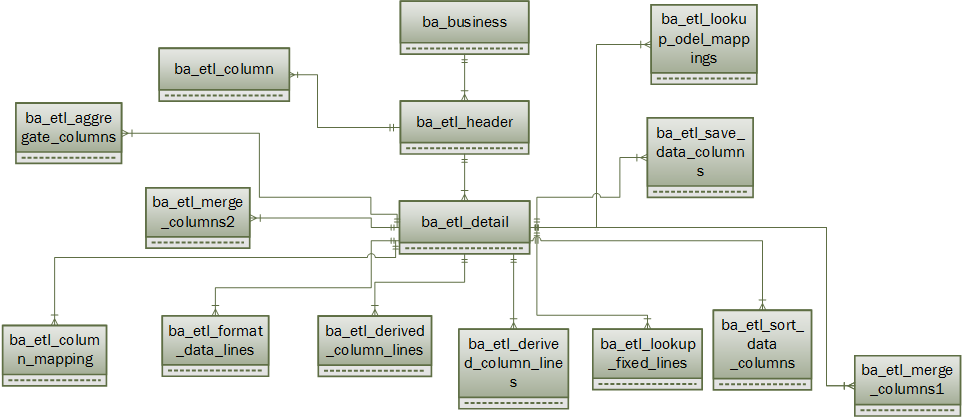
\includegraphics[scale=0.6]{Gambar/Pemodelan-Basisdata}
	\caption{Struktur tabel BI \textit{tool}}
	\end{figure}

Berikut ini penjelasan mengenai pemodelan basisdata dari BI \textit{tool}
\begin{enumerate}
	\item \textbf{ba\_bussiness} : Tujuan pembuatan tabel ini adalah supaya banyak perusahaan/bisnis yan dapat menggunakan \textit{tool} ini (\textit{multicompany/multiclient}).
	\item \textbf{ba\_etl\_header} : Berfungsi sebagai list proses ETL yang ada di bawah perusahaan tersebut.
	\item \textbf{ba\_etl\_detail} : Menyimpan detil setiap proses ETL di bawah perusahaan tersebut.
	\item \textbf{ba\_etl\_columns}: Kolom-kolom yang terlibat di dalam proses ETL, baik dari \textit{file} sumber data maupun yang ditambahkan di tengah proses.
	\item \textbf{ba\_etl\_columns\_mapping} : Detil \textit{mapping} kolom dari data \textit{input} ke \textit{output}. Dimana user bisa memilih untuk tetap memakai nama kolom lama atau mengubahnya.
	\item \textbf{ba\_etl\_format\_data\_lines} : Khusus tipe ETL \textit{format} data menyimpan detil informasi, tipe, dll dari setiap kolom.
	\item \textbf{ba\_etl\_sort\_data\_columns} : Khusus tipe ETL \textit{sort data} menyimpan detil informasi kolom dan arah sorting.
	\item \textbf{ba\_etl\_derived\_column\_lines} : Khusus tipe ETL \textit{derived column} menyimpan detil formula untuk menghasilkan \textit{derived column}.
	\item \textbf{ba\_etl\_lookup\_fixed\_lines} : Khusus tipe ETL \textit{lookup} menyimpan bila \textit{lookup} diambil dari himpunan pilihan \textit{fixed}, tabel ini menampung piluhan-pilihan tersebut.
	\item \textbf{ba\_etl\_save\_data\_columns} : Khusus tipe ETL \textit{save data} menyimpan \textit{mapping} kolom antara hasil dari proses ETL dengan \textit{field} di tabel.
	\item \textbf{ba\_etl\_lookup\_model\_mappings} : Khusus tipe ETL \textit{lookup} menyimpan bila lookup diambil dari tabel lain, tabel ini menampung pasangan \textit{field} di data proses dengan yang di tabel \textit{lookup}.
	\item \textbf{ba\_etl\_merge\_columns1} : Khusus tipe ETL \textit{merge} menyimpan informasi \textit{merge} dari sumber pertama.
	\item \textbf{ba\_etl\_merge\_columns2} : Khusus tipe ETL \textit{merge} menyimpan informasi merge dari sumber kedua
	\item \textbf{ba\_etl\_aggreagate\_columns} : Khusus tipe ETL \textit{aggregate} menyimpan detil informasi proses \textit{aggregate} 
	
\end{enumerate}




















	
